\chapter{Efficient Transfer of Knowledge for Deep Hedging of Variable Annuities}

\section{Introduction}

Reinforcement Learning (RL) is a branch of machine learning that focuses on training algorithms, known as agents, to make a sequence of decisions. 
The agent learns to achieve a goal in an uncertain, potentially complex environment by trial and error, using feedback from its own actions and experiences. 
Unlike supervised learning, where training data is labeled with the correct answers, in RL, an agent is provided with rewards or punishments as signals for its actions.

The core of RL revolves around the concept of the agent interacting with its environment over time, aiming to maximize the cumulative reward. 
This process involves observing the state of the environment, selecting and performing actions, and receiving rewards or penalties in response to those actions. 
The agent's objective is to learn a mapping from states to actions that maximizes this cumulative reward, which is often referred to as a policy. 
One of the fundamental frameworks for modeling RL problems is the Markov Decision Process (MDP). 
An MDP provides a mathematical formulation of the decision-making process, characterized by states, actions, rewards, and transition probabilities. Solving an MDP involves finding a policy that maximizes some function of the expected rewards, typically the expected cumulative reward over time.

Reinforcement learning algorithms can be broadly categorized into two types: model-based and model-free approaches. 
Model-based methods utilize a model of the environment to simulate the outcomes of actions, enabling planning and decision-making with fewer interactions with the environment. 
Conversely, model-free methods learn directly from interactions with the environment, without relying on a model, making them more straightforward but often less efficient in terms of sample usage.

A compelling application of RL is in the hedging of financial derivatives, a domain where the complexity and uncertainty of financial markets make traditional static models inadequate.
Financial derivatives are contracts whose value is derived from an underlying asset, and hedging is the practice of making investments to reduce the risk of adverse price movements.
RL's adaptability and learning capabilities offer a promising solution to dynamically adjust hedging strategies in response to market movements.
This approach, particularly with model-free algorithms, has the potential to enhance risk management practices by developing strategies that can adapt in real-time to changing market conditions.

In this paper, we propose a transfer learning approach to improve the risk management of variable annuities (VAs) by learning a hedging strategy utilizing previous experiences from other financial products.
VAs are popular retirement products that combine investment and insurance features, offering policyholders the potential for investment growth and the protection of a guaranteed minimum death benefit or income benefit.
Due to the complexity of the products and the dynamic nature of the financial markets, the task of hedging VAs is particularly challenging.
We aim to leverage the knowledge from the hedging strategies of financial derivatives to construct hedging strategies for VAs, thereby improving the risk management of these products.
The rest of the paper is organized as follows: Section~\ref{sec3:vaHedging} presents the problem formulation for hedging variable annuity with a deep neural network, Section~\ref{sec3:tlHedging} presents the background knowledge for transfer learning, and Section~\ref{sec3:numerical} states the plans for ongoing numerical experiments.

\section{Dynamic Hedging of Variable Annuities} \label{sec3:vaHedging}

\subsection{Markov Decision Process (MDP) for Hedging VAs}
A Markov Decision Process (MDP) provides a mathematical framework for solving sequential decision-making tasks in situations where outcomes are partly random and partly under the control of an agent. 
In the context of hedging VAs, an MDP can be used to model the decision-making process of an insurer who aims to minimize the liability of the VA by dynamically adjusting the hedging portfolio based on the current state of the VA and the financial markets.
An MDP is defined by the tuple $\mathcal{M} = (\mu_0, \mathcal{S}, \mathcal{A}, \mathcal{P}, \mathcal{R}, \gamma)$, where:

\begin{itemize}
    \item $\mu_0$ is the initial states.
    \item $\mathcal{S}$ is a finite set of states.
    \item $\mathcal{A}$ is a finite set of actions.
    \item $\mathcal{P}$ is a state transition probability distribution, where $\mathcal{P}(s'|s, a)$ represents the probability of transitioning from state $s$ to state $s'$ due to action $a$.
    \item $\mathcal{R}$ is a reward distribution, $\mathcal{R}(s, a, s')$ is the reward received after transitioning from state $s$ to state $s'$ due to action $a$.
    \item $\gamma$ is a discount factor, $\gamma \in [0,1]$,  which models the present value of future rewards.
\end{itemize}

The objective in an MDP is to find a policy, $\pi: \mathcal{S} \rightarrow \mathcal{A}$, that maximizes the cumulative reward over time, often referred to as the value function for a policy $\pi$ at state $s$: 

\begin{equation} \label{eq3:V_pi}
    V^{\pi}_{\mathcal{M}}(s) = \mathbb{E}_{s_0 \sim \mu_0, a_i \sim \pi(\cdot|s_i), s_{i+1} \sim \mathcal{P}(\cdot|s, a)} \left[ \sum_{t=0}^{\infty} \gamma^t R_{t+1} |\pi, s \right],
\end{equation}

where $R_{t+1} = \mathcal{R}(s_i, a_i, s_{i+1})$ is the reward received by the agent after taking action $a_i$ in state $s_i$ and transitioning to state $s_{i+1}$, and the expectation is taken over the possible sequences of states and rewards that follow from the policy $\pi$.
In the context of hedging VAs, the initial states $\mu_0$ specifies the initial value of the VA and the market specifications. 
The state space $\mathcal{S}$ represent the information available to the agent, such as current value of the underlying asset ($S_t$), the current subaccount value ($F_t$), and the guarantee value ($G_t$), as well as other relevant contract specifications.
The action space $\mathcal{A}$ represent the hedging decisions, such as the hedging portfolio weights.
The state transition probability distribution $\mathcal{P}$ and the reward function $\mathcal{R}$ are derived from the dynamics of the VA and the market specifications. Instead of having an infinite time horizon, the final reward is obtained at the maturity of the VA contract. Hence, $R_{t} = 0$ for all $t > T$.
The discount factor $\gamma$ models the present value of future rewards and is conveniently inherited from the risk-free rate. 

Considering the task of hedging a GMWB contract, the hedging strategy aims to minimize the insurer's liability $L_t$ at each time $t=1,\ldots,T$ by dynamically adjusting the hedging portfolio based on the current state of the VA and the financial markets. The objective is to find a policy $\pi$ that minimizes the expected liability over time, i.e., 

\begin{equation}
    \min_{\pi} \mathbb{E}[\sum_{t=1}^{T} \gamma^t L_t | \pi, s_0],
\end{equation}

where it can be conveniently rewritten as the value function $V^{\pi}_{\mathcal{M}}(s)$ in Equation~\ref{eq3:V_pi} by setting the reward function $R_{t} = -L_t$ and the discount factor $\gamma = \frac{1}{1+r}$. 
Other value functions can be used to optimize over a risk measure on the cumulative liability, such as the Value-at-Risk (VaR) or the Conditional Value-at-Risk (CVaR).
Denote the risk measure as $\rho_{\alpha}$, where $\alpha$ is the confidence level, then the value function can be set as

\begin{equation}
    V^{\pi}_{\mathcal{M}}(s) = \rho_{\alpha}(\sum_{t=1}^{T} \gamma^t L_t | \pi, s_0).
\end{equation}

\subsection{Deep Hedging Approaches}

Deep hedging is a reinforcement learning approach that leverages deep learning models to optimize hedging strategies for financial derivatives.
In deep hedging, the objective is to minimize the hedging error or a risk measure over a set of paths of the underlying asset, which involves training the DNNs using backpropagation and optimization algorithms to find the hedging strategy that maximizing the value function.

\begin{enumerate}
    \item \textbf{Value Function:} Specify a value function that quantifies the hedging performance. 
    This could include minimizing the expected liability, the CVaR, or the variance of portfolio returns.
    \item \textbf{Training and Optimization:} Using historical data or simulated data generated from the specified market model, train the DNN using backpropagation and optimization algorithms to find the hedging strategy that maximizes the value function.
    \item \textbf{Implementation and Adjustment:} Implement the learned hedging strategy in real-time trading, with periodic adjustments based on new market information and continuous learning to adapt to changing market dynamics. This is often referred to as online learning.
\end{enumerate}

Depending on the specific market model and the hedging objective, deep hedging can be categorized into model-based and model-free approaches.
Model-based deep hedging trains a deep neural network (DNN) to learn optimal hedging actions by maximizing a value function that reflects the hedging error or risk measure, such as the variance of the hedging portfolio's final value or tail risk measures like the CVaR.
The DNN processes sequential market data and outputs a policy that determines the hedging actions based on the current state of the market.
In the context of deep hedging, the policy $\pi = \phi(\mathcal{I})$ is defined by the parameter $\phi$ of a DNN, and the information $\mathcal{I}$ is the training data during the learning process.
~\cite{buehler2019deep} is the first paper to propose a model-based deep hedging approach for hedging financial derivatives with a focus on minimizing CVaR.
A more recent paper by~\cite{imaki2021no} proposes a new network architecture for model-based deep hedging that can be trained more efficiently.
A typical setup for a model-based deep hedging strategy includes:

\begin{enumerate}[label=\arabic*a.]
    \setcounter{enumi}{3}
    \item \textbf{Market Model Specification:} Define the underlying asset price dynamics and the risk factors affecting the financial instruments. Common models include geometric Brownian motion for stock prices or more complex models accounting for jumps or stochastic volatility.~\cite{glasserman2004monte} provides detailed discussions on simulating asset prices under various models.
    \item \textbf{Deep Neural Network Design:} Design a DNN architecture capable of processing sequential market data and making hedging decisions. The network outputs a policy by receiving inputs that include historical prices, option strikes, and other relevant financial indicators.~\cite{buehler2019deep} uses a feedforward neural network (FNN), where its input layer receives the current state of the market, and its output layer produces the hedging weights.
\end{enumerate}

Conversely, model-free deep hedging approaches directly learn from historical market data without making explicit assumptions about asset price dynamics. 
Instead, the value functions are learned directly from the data, and the hedging strategies are derived from the learned value functions.
A typical setup for a model-free deep hedging strategy includes:

\begin{enumerate}[label=\arabic*b.]
    \setcounter{enumi}{3}
    \item \textbf{Market Model Specification:} No explicit model assumptions are made about the underlying asset price dynamics. Instead, the deep learning model learns the value function and hedging strategies directly from historical market or simulation data.
    \item \textbf{Deep Neural Network Design:} Design two DNNs: a value network and a policy network. The value network learns the value function, while the policy network learns the optimal hedging actions based on the approximated value function.
\end{enumerate}

A model-free approach does not require explicit model assumptions about asset price dynamics, making it more flexible and adaptable to different market conditions and more robust to model misspecification.

\subsection{Value-based and Policy-based Deep Reinforcement Learning}

Model-free deep reinforcement learning algorithms can be broadly categorized into two types: value-based and policy-based approaches.

\begin{enumerate}
    \item \textbf{Value-based Deep Reinforcement Learning:} Value-based approaches learn the value function directly from the data and derive the policy from the learned value function. 
    The value function is learned by training a DNN to approximate the value function, which quantifies the expected cumulative reward over time. 
    The policy is then derived from the learned value function by selecting the action that maximizes the value function at each state. 
    ~\cite{mnih2015human} is the first paper to demonstrate the effectiveness of value-based deep reinforcement learning in training agents to play Atari games.
    To update the value function, the DNN is trained to minimize the difference between the current value function and the target value function, which is updated based on the maximum expected reward from the previous iteration.
    When trained to approximate the value function, the DNN benefits from the use of experience replay buffers, which is proposed by~\cite{lin1992self} to store and sample historical transitions and uniformly sampled during training to enhance the sample efficiency and stability of the learning process.
    ~\cite{kolm2019dynamic} uses a value-based deep reinforcement learning approach to hedge European options under the Black-Scholes framework.

    \item \textbf{Policy-based Deep Reinforcement Learning:}
    In valued-based approaches, the value function is updated iteratively with the maximum expected reward of all possible actions, which can be computationally expensive for continuous action spaces.
    To overcome this difficulty, a policy-based approach estimates the value function before realization of the final payoff of the hedging portfolio, which is particularly useful for hedging long-term financial derivatives or VA contracts.
    Two types of policy-based approaches prevail in the literature: actor-critic and policy gradient methods.

    An actor-critic method designs an actor network and a critic network to learn the value function and the policy simultaneously.
    The actor network learns the policy by directly outputting the action based on the current state, while the critic network learns the value of an action by approximating the expected cumulative reward over time following the actor's policy.
    A popular actor-critic algorithm is the Deep Deterministic Policy Gradient (DDPG) algorithm proposed by~\cite{lillicrap2015continuous}, which is implemented by~\cite{xu2022delta} in hedging financial derivatives in S\&P 500 and DJIA index options.
    
    A policy gradient method uses policy gradient theorem to update the policy by performing gradient ascent with respect to the policy parameters.
    Representative algorithms include the Proximal Policy Optimization (PPO) algorithm proposed by~\cite{schulman2017proximal} and the Trust Region Policy Optimization (TRPO) algorithm proposed by~\cite{schulman2015trust}.
    The most relevant paper to our study is~\cite{chong2023pseudo}, which uses the PPO algorithm to hedge GMMB with a GMDB rider under the Black-Scholes framework.
\end{enumerate}

\section{Transfer Learning for Risk Management of Variable Annuities} \label{sec3:tlHedging}

Transfer learning is a machine learning technique that leverages knowledge from one domain to improve learning in another domain.
In the context of deep reinforcement learning, transfer learning can be used to improve the risk management of VAs in five ways:
\begin{enumerate}
    \item   \textbf{Transferring to VA products}: Knowledge can be transferred from the hedging strategies of financial derivatives to constructing hedging strategies for VAs.
    VAs are complex insurance products with unique features, which makes it challenging to develop effective hedging strategies.
    However, the payoff structures of VAs are similar to those of financial derivatives, such as European options, which have been extensively studied in the literature.
    By leveraging the knowledge from the hedging strategies of financial derivatives, we can improve the risk management of VAs.
    \item   \textbf{Transferring to new VA products}: Knowledge can be transferred from the hedging strategies of one VA product to another VA product.
    Different VA products have different features and payoff structures, which makes it challenging to develop hedging strategies for new VA products.
    However, experience from hedging one VA product can be transferred to develop hedging strategies for new VA products, especially when the new VA product is similar to the existing ones.
    \item   \textbf{Transferring to new asset models}: Knowledge can be transferred from the hedging strategies of one asset model to another asset model.
    A stochastic volatility model is a more realistic model for asset prices than the Black-Scholes model, but it is more challenging to develop hedging strategies for VAs under such a model.
    \item  \textbf{Transferring to new model specifications}: Model misspecification is a common issue in financial modeling, and training on data simulated with misspecified parameters can lead to suboptimal hedging strategies.
    If only the misspecified model is similar to the correct model, then we can leverage the knowledge from the misspecified model to improve the hedging strategies under the correct model, since the only difference between the two models is the parameter values. 
    \item   \textbf{Transferring to the real world}: Knowledge can be transferred from simulated data to real-world data.
    In practice, it is challenging to obtain real-world data for VAs, but we can leverage simulated data to develop hedging strategies for VAs.
    If the simulated data is representative of the real-world data, then the hedging strategies developed from the simulated data can be transferred to the real world.

\end{enumerate}

Given a set of source domains $\bm{\mathcal{M}}_s= \{ \mathcal{M}_s| \mathcal{M}_s \in \bm{\mathcal{M}}_s\}$ and a target domain $\mathcal{M}_t$, transfer learning aims to improve the learning on the target domain.
While utilizing the interior information $\mathcal{I}_t$ from the target domain, the exterior information $\mathcal{I}_s$ from the source domains is also leveraged to improve the learning on the target domain.

\begin{equation}
    \pi^* = \arg \max_\pi \mathbb{E}_{s \sim \mu_0, a \sim \pi} \left[V_{\mathcal{M}}^\pi (s, a) \right], 
\end{equation}

where $\pi = \phi(\mathcal{I}_s \sim \bm{\mathcal{M}}_s, \mathcal{I}_t \sim \mathcal{M}_t)$ is policy learned from target domain based on information from both the source domains and the target domain.
A regular reinforcement without transfer learning is a special case where $\mathcal{I}_s = \emptyset$ and $\pi = \phi(\mathcal{I}_t \sim \mathcal{M}_t)$.

In the context of deep hedging, various research has been conducted to improve the hedging strategies on real-world data by leveraging knowledge from simulated data.
Most of the research uses the offline-online learning approach, where the hedging strategies are first trained with simulation data, but updated in real-time based on new market information and continuous learning to adapt to changing market dynamics.
The most relevant paper to our study is~\cite{xiao2021optimal}, which use policy gradient algorithms to train hedging strategies for European options with simulation data from Heston model and then updated in real-time hedging S\&P 500 index options.
To the best of our knowledge, no research has been conducted to improve the hedging strategies with the state-of-the-art transfer learning techniques.
This section introduces some transfer learning techniques that are relevant to our task of hedging VAs.

\subsection{Reward Shaping}

In the context of hedging VAs using deep reinforcement learning and transfer learning, reward shaping becomes a crucial technique. 
It involves modifying the reward function in the target domain to incorporate additional guidance, which often leads to more efficient learning and better performance.
This technique can be particularly useful for managing the complex risks associated with VAs, as it can guide the learning process towards strategies that are more effective in hedging these products.

One way to implement reward shaping in this context is by introducing auxiliary rewards that reflect the performance of hedging strategies learned from the source domains.
Reward shaping learns an auxiliary reward function $\mathcal{R}_s: \mathcal{S} \times \mathcal{A} \times \mathcal{S} \rightarrow \mathbb{R}$ from the source domains.
The auxiliary reward function is then used to shape the reward function in the target domain, $\mathcal{R}'_t = \mathcal{R}_t + \mathcal{R}_s$, by incorporating the insights gained from the source domains.

Some popular reward shaping techniques include potential-based reward shaping~\citep{ng1999policy}, potential based state-action advice~\citep{wiewiora2003principled}, dynamic value function advice~\citep{harutyunyan2015expressing}.

\subsection{Policy Transfer}

The most straightforward approach to transfer learning is to directly transfer the policy learned from the source domains to the target domain via policy distillation.
Policy distillation is a technique that transfers the knowledge from a teacher policy to a student policy by training the student policy to mimic the teacher policy up to a certain extent.
The teacher policy is learned from the source domains, and the student policy learns the hedging strategies in the target domain while guided by the teacher policy.
In the Distral algorithm~\citep{teh2017distral}, the student policy maximizes a multi-task objective:
$\max_{\phi} \sum_{i=1}^K \mathcal{J}(\pi_\phi, \pi_{E_i})$, where

\begin{equation}
    \mathcal{J}(\pi_\phi, \pi_{E_i}) = \sum_{t=0}^\infty \mathbb{E}_{s_t \sim \mu_0^t, a_t \sim \pi_\phi} \left[ \gamma^t R_{t+1} + \frac{\alpha}{\beta} \log \pi_{\phi}(a_t|s_t) - \frac{1}{\beta}log \pi_{E_i}(a_t|s_t) \right],
\end{equation}

where a set of $K$ teacher policies $\pi_{E_i}$ are learned from the source domains, and the student policy $\pi_\phi$ is learned on the target domain. $\alpha$ and $\beta$ are hyperparameters that control the trade-off between mimicking the teacher policies and exploring the target domain.

\subsection{Representation Transfer}

Representation transfer is a technique that transfers the knowledge based on the following critical assumption:

\begin{assumption}
    The state space $\mathcal{S}$, the action space $\mathcal{A}$, and the reward function $\mathcal{R}$ can be disentangled into orthogonal subspaces, which are task-invariant such that knowledge can be transferred between domains on the universal subspaces.
\end{assumption}

A suitable representation transfer technique for our task of hedging VAs is modular networks~\citep{andreas2017modular}, which decomposes a policy $\pi$ into two sub-modules $g$ and $f$, i.e.,

\begin{equation}
    \pi = \phi(s_{market}, s_{guarantee}) = f(g(s_{market}), s_{guarantee}),
\end{equation}

~\cite{zhang2018decoupling} uses modular networks to transfer knowledge of physics models from previous tasks to new tasks in a simulated environment.
In the context of hedging VAs, $g$ is the module that processes the market information, and $f$ is the module that processes the guarantee information.
The core idea behind modular networks is that the market information can be applied for hedging strategies across different VA products, while the guarantee information is specific to each VA product.
Hence, knowledge can be transferred from the source domains to the target domain by transferring the market module $g$.

\subsection{Evaluation Metrics}

The metrics discussed for evaluating transfer learning approaches focus on two key aspects: mastery and generalization. 
Mastery assesses the agent's final performance level in the target domain, indicating how effectively it has learned a specific task from previous knowledge. 
Some common metrics for evaluating mastery include:

\begin{itemize}
    \item \textbf{Asymptotic performance:} the final reward of the agent in the target domain.
    \item \textbf{Transfer ratio:} the ratio of the agent's performance in the target domain with and without transfer learning.
\end{itemize}

Generalization, on the other hand, refers to the agent's ability to quickly adapt its learned knowledge to the target domain.

\begin{itemize}
    \item \textbf{Jumpstart performance:} the initial reward of the agent in the target domain.
    \item \textbf{Accumulated reward:} the total area under the reward curve over time in the target domain.
    \item \textbf{Time to threshold:} the time it takes for the agent to reach a certain performance threshold in the target domain.
    \item \textbf{Performance with fixed epochs:} the agent's performance in the target domain after a fixed number of epochs.
\end{itemize}

\section{Plans for Ongoing Numerical Experiments} \label{sec3:numerical}

As we aim to enhance the risk management strategies for variable annuities (VAs) through the application of transfer learning, our next step involves conducting a series of numerical experiments. These experiments are crucial for validating the theoretical frameworks and methodologies developed so far. Our plan includes:

\begin{enumerate}
    \item \textbf{Simulation setup:} Designing a simulation environment that closely mirrors real-world market dynamics and VA contract specifics. 
    This setup will include various asset models, including the Black-Scholes and stochastic volatility models, to test the adaptability of transferred hedging strategies across different market conditions.
    \item \textbf{Baseline model comparison:} Establishing a set of baseline hedging strategies against which we can compare the performance of our transfer learning-enhanced strategies. 
    This will likely involve traditional delta hedging techniques and possibly other reinforcement learning approches that have not utilized transfer learning.
    \item \textbf{Transfer learning implementation:} Applying the transfer learning methodologies discussed, including reward shaping, policy transfer, and/or representation transfer to the task of hedging VAs. 
    The transfer can happen between different VA products, different asset models, different model specifications, and between simulated and real-world data.
    \item \textbf{Performance evaluation:} Utilizing the evaluation metrics outlined in the previous sections to assess mastery and generalization of the transfer learning strategies. 
    Key metrics will include asymptotic performance, transfer ratio, jumpstart performance, and time to threshold.
    \item \textbf{Sensitivity analysis:} Conducting sensitivity analyses to understand how changes in market conditions, contract specifics, and model parameters affect the performance of our transfer learning strategies. This will help in identifying the robustness and limitations of our approach.
    \item \textbf{Hedging in real-world:} If accessible, applying the trained models to real-world data to further validate their practical applicability and performance in real-world market conditions.
\end{enumerate}

Through these numerical experiments, we aim to demonstrate the efficacy of transfer learning in improving the hedging of VAs in a variety of market conditions and contract specifics. 
We expect that our transfer learning-enhanced strategies will outperform traditional hedging techniques and possibly other machine learning approaches that have not utilized transfer learning. 
This will provide strong evidence for the potential of transfer learning in improving risk management strategies for VAs and other complex financial products in a dynamic market environment.

\subsection{Initial Numerical Experiments}

\begin{figure}[ht!]
    \centering
    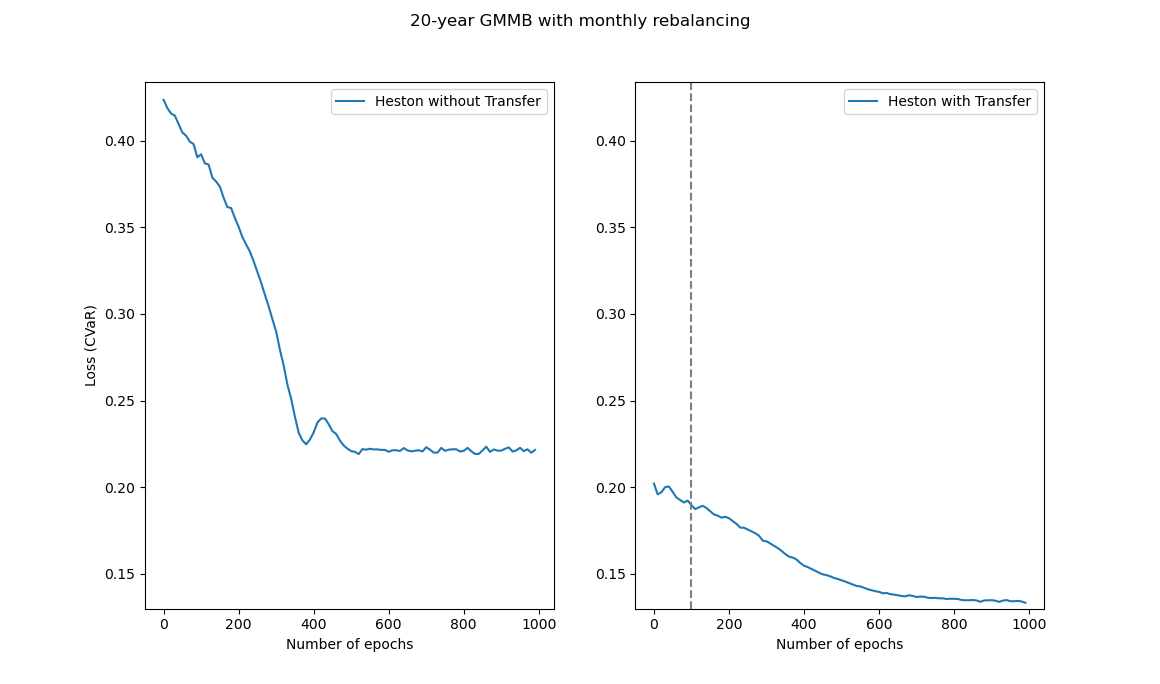
\includegraphics[width=0.8\textwidth]{./project3/figures/Figure_1.png}
    \caption{Initial numerical experiments for GMMB}
    \label{fig3:GMMB}
\end{figure}

